En esta sección haremos un breve repaso de las funcionalidades provistas por \texttt{Manticore}.
Luego podremos discernir dadas estas funcionalidades la mejor estrategia para utilizar \texttt{Manticore} como el back end de la construcción de EPAs.
Toda esta sección se refiere a la versión de \texttt{Manticore 0.3.7}.

\texttt{Manticore} es un proyecto desarrollado por \texttt{TrailOfBits} lanzado en 2017.
Es una herramienta de ejecución simbólica, implementada en Python, que soporta análisis para diversas plataformas: EVM, bytecode nativo (arquitecturas \texttt{x86}, \texttt{x86\_64}, \texttt{aarch64} y \texttt{ARMv7}) y WASM.
Principalmente funciona como un motor de ejecución simbólica programable (mediante APIs externas en Python), aunque también incluye una herramienta plug-and-play por línea de comandos, y existe un proyecto que intenta integrar la herramienta con una interfaz gráfica, \texttt{ManticoreUI} \cite{manticoreUI} que nunca se lanzó.

\section{Herramienta por Línea de Comandos}

El comportamiento por defecto de la herramienta de línea de comandos varía mucho dependiendo de la plataforma \footnote{la sugerencia pregunta qué es plataforma pero dice el parrafo anterior. ¿Qué no se entiende?} a la que es aplicada, pero en general busca explorar todos los caminos de ejecución factibles en el código fuente provisto, utilizando valores simbólicos para cada valor generalmente introducido por usuarios.
Luego, por cada camino explorado, genera un caso de test (es decir, genera un valor concreto que fuerze el camino para cada valor ``input'' simbólico).
Además, la exploración de los caminos incluye el seguimiento de algunas propiedades interesantes por defecto, dependientes de la plataforma.
Para los binarios nativos, por ejemplo, registra el conjunto (total) de instrucciones visitadas, y registra para cada caso de test el número y la traza exacta de instrucciones ejecutadas.

En el caso de la EVM, la herramienta por consola funciona con código fuente Solidity (no acepta precompilados).
Para explorar caminos de ejecución la herramienta toma los métodos externos del contrato y los ejecuta (en cualquier orden) hasta alcanzar 100\% de line coverage o, dentro de un límite si es que se introdujo uno, hasta cubrir todo el espacio de secuencias de llamados a métodos externos.
De no alcanzar ninguno de estos dos criterios, termina el análisis por time out.
La herramienta cuenta con una batería de \texttt{detectors} que registran eventos de  interés específico a Ethereum, como la presencia de integer overflows, la ejecución de opcodes inválidos, la lectura de memoria o storage no inicializado, bugs de reentrancy o la ejecución de ciertas instrucciones específicas con parámetros controlados por el usuario.
Estos \texttt{detectors} se encuentran apagados por defecto, al igual que por defecto se descartan caminos que incluyan el rollback de una transacción.
Esto significa que, por ejemplo, para realizar una simple búsqueda de incumplimiento de una aserción (la instrucción \textcolor{blue}{\texttt{assert}} en Solidity), es preciso activar el modo detallado (\texttt{--thorough-mode}) de la herramienta \footnote{la sugerencia es agregar un ejemplo pero ya siento que es un detalle muy insigificante esto. Además, ¿que sería un ejemplo? ¿un contrato con un assert falseable? ¿para qué? }.

\section{Manticore-Verifier}
Manticore cuenta con otra herramienta por consola de comandos de análisis de smart contracts denominada \texttt{manticore-verifier}.
Permite marcar ciertos métodos externos como ``invariantes'' que la herramienta luego busca falsificar.
Una fortaleza de esta herramienta es que la sintaxis para marcar los invariantes es la misma que la utilizada por \texttt{Echidna}, un fuzzer desarollado también por \texttt{TrailOfBits} \cite{echidna}, permitiendo el análisis por ambas herramientas con una única intervención manual.

\section{Arquitectura}
La arquitectura de Manticore se organiza en tres partes:
\begin{itemize}
    \item El mecanismo central de ejecución simbólica
    \item Los módulos que implementan la simulación de cada una de las plataformas soportadas (Ethereum, \texttt{x86}, etc)
    \item SMT solvers externos
\end{itemize}

Por defecto, la instalación de Manticore incluye una instalación del \texttt{Z3 Theorem Prover}, un SMT solver desarrollado por Microsoft Research desde 2012 \cite{z3TheoremProver}.
Sin embargo, Manticore puede integrarse con cualquier SMT solver que se conforme a la interfaz definida por \texttt{SMTLIB2} \cite{smtlib2}, como lo es por ejemplo también \texttt{Yices} \cite{yices}, otro SMT solver open source.

El mecanismo central de ejecución simbólica de Manticore está compuesto por varios módulos de Python: \texttt{\textbf{smtlib}}, \texttt{\textbf{manticorebase}}, \texttt{\textbf{plugin}}, \texttt{\textbf{state}}, \texttt{\textbf{worker}} y \texttt{\textbf{workspace}}, representados en la figura \ref{fig:core-modules}.

\begin{figure}
    \centering
    {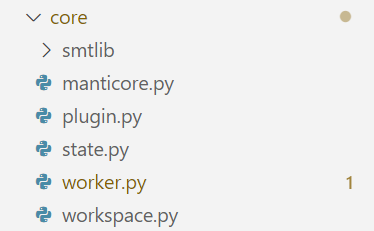
\includegraphics {figs/core-architecture-manticore.png}}
    \caption{Módulos que componen el mecanismo central de ejecución simbólica de Manticore}
    \label{fig:core-modules}
\end{figure}

\texttt{\textbf{smtlib}} provee a los demás módulos de la aplicación APIs para generar y manipular variables, expresiones y constraints simbólicas, y para realizar consultas de (in)satisfacibilidad sobre las expresiones simbólicas generadas, delegando estas consultas en última instancia al SMT solver externo.
Los módulos \texttt{\textbf{manticorebase}} y \texttt{\textbf{state}} implementan en conjunto el mecanismo central de ejecución simbólica de Manticore asumiendo lo mínimo posible sobre las instrucciones emuladas \footnote{Es decir, sobre la plataforma que use el programa que se está analizando}.
Por último, \texttt{\textbf{worker}} y \texttt{\textbf{workspace}} sirven de auxiliares que soportan los aspectos de perstistencia, entrada/salida y multithreading, entre otros, de la aplicación.
El módulo \texttt{\textbf{plugin}} provee una API de \textit{callbacks} que otorgan acceso al estado interno emulado en distintos momentos de la ejecución.
Este módulo es una parte central de la API programable accesible al usuario de Manticore, pero también es la manera en la que la aplicación base puede realizar sus análisis de coverage, etc.

La abstracción principal para la ejecución simbólica utilizada por Manticore es la del objeto \textcolor{cyan}{\texttt{state}}.
Un \textcolor{cyan}{\texttt{state}} representa, habiendo realizado un camino de ejecución particular, el estado del programa emulado hasta cierto punto.
Los \textcolor{cyan}{\texttt{state}} son responsables de conocer cuáles son los próximos pasos en su ejecución, cuál es el conjunto de variables simbólicas que existieron en su ejecución, y qué conjunto de fórmulas deben satisfacerse.
Asimismo, cada \textcolor{cyan}{\texttt{state}} individual cuenta con una instancia entera emulada del programa (en el caso de Ethereum, la blockchain).
Por otro lado, el estado global de la aplicación (mantenido por el módulo \texttt{\textbf{manticorebase}}) consiste simplemente en una colección de \textcolor{cyan}{\texttt{state}}.

\section{API programable}
\label{sec:api-manticore}
La principal API presentada al usuario permite manejar el conjunto global de \textcolor{cyan}{\texttt{state}}s, siempre ``entre medio'' de la ejecución de métodos del contrato (es decir, antes de comenzar a ejecutarlos o después de que terminen, pero no durante).
Los principales métodos de la API permiten realizar acciones globales como introducir nuevas constraints, ejecutar métodos de un smart contract, deployear un contrato nuevo, o iniciar la generación de casos de test a partir de los \textcolor{cyan}{\texttt{state}}.
Además, permiten acceder a \textcolor{cyan}{\texttt{state}} individuales (siempre y cuando no estén corriendo) y leer y/o modificar los elementos simbólicos de su estado.
Sin embargo, al menos mediante la API expuesta, no es posible expandir el camino de ejecución de sólo algunos \textcolor{cyan}{\texttt{state}}.
Esto siempre debe hacerse mediante la ejecución de métodos externos al nivel más alto, afectando a todos los \textcolor{cyan}{\texttt{state}} \footnote{``Agregar un ejemplo si es posible (textual)'' --- ¿Que significa??}.

Por otro lado los callbacks como los del módulo
\texttt{\textbf{plugin}} permiten interactuar con los \textcolor{cyan}{\texttt{state}} mientras estos se ejecutan.
Los callbacks pueden suscribirse a cualquiera de los eventos publicados nativamente por la aplicación, que son de naturaleza muy amplia y granularidad diversa, en lugar de simplemente eventos que modifiquen el estado de los \textcolor{cyan}{\texttt{state}}.
Algunos de los eventos pueden categorizarse en:
\begin{itemize}
    \item eventos de estado (\texttt{will\textbackslash did\_fork\_state, will\textbackslash did\_terminate\_state})
    \item eventos de smt (\texttt{will\textbackslash did\_solve})
    \item eventos de plataforma (\texttt{will\textbackslash did\_open\_transaction},\\ \texttt{will\textbackslash did\_evm\_read\_storage})
\end{itemize}
Estos pueden utilizarse para debugear o mantener el registro de propiedades, pero también para modificar el estado de la ejecución en vivo.


